\chapter{Evaluation}

With the eventual growth of the Lightning Network a fee market for channel liquidity will emerge. In this chapter the dynamics by which this fee market operates are sought. Strategies and routing node behavior are suggested in an effort to create a simulation where strategies can be tested against each other. 

\section{Lightning network as a graph}

The Lightning Network may be modeled as a directional Graph $G$ with vertices representing nodes and edges representing channels. As each channel may have different fees and liquidity in each direction it's useful to represent each channel with two edges. One edge in each direction. 

\begin{figure}[!htb]
	\hspace*{-0.7cm} 
	\centering
	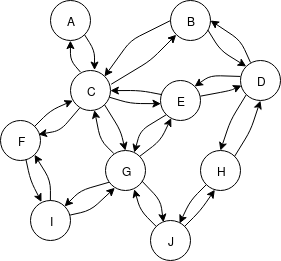
\includegraphics[width=7cm]{images/LN_overview.png}
	\caption{ \textit{A representation of LN as a graph. Each channel is symbolized by two edges.} 
	}
	\label{fig:ln:graph}
	\hspace*{2mm}
\end{figure}

Modeling the network as a graph allows the use of graph theory. Thus routing, concepts of centrality and analytical frameworks may be borrowed from the extensive literature on graphs. The topology of both Testnet and Mainnet is visualized in Figure \ref{fig:topology}.

\section{Fee as a competitive equilibrium}

It may be useful to view the fee market as existing under normal free market pressures and apply the conventional long run demand and supply curve~\cite{boulding:evolutionary:economy} to the fee market. 

\begin{figure}[!htb]
	\hspace*{-0.3cm}
	\centering
	\includegraphics[width=11cm]{images/equilibrium_sized2.png}
	\caption{ The fee market as viewed according to standard price theory. Both by single pair and all pairs in aggregate. 
		}
		\label{fig:equilibrium}
		\hspace*{2mm} 	
\end{figure}

The demand curve DD' signifies users demand to utilize a shortest path in the lightning network and the supply curve the existing competing paths between s and d. Say there exists a Equilibrium point E by with the market price will move towards. Suppose the average fee price is greater than equilibrium at $F_{1}$ with demand $F_{1}D_{1}$ and supply $F_{1}S_{2}$, and more operators would open a path between s and d driving the curve fee towards E. If it instead lay under the equilibrium at $F_2$ their would be an excess supply $F_{2}S_{1}$ and low demand $F_{2}D_{2}$, making operators loose money by having liquidity locked up on a path not used. Thus leading operators to close channels between s and d, again driving the fee towards E.

The fee market may also be seen in its aggregate, where the axis represents the whole network. Here the drivers might be seen as new routing nodes joining if its a profitable venture or leaving if its a unprofitable one. Here again driving prices towards equilibrium. 

It may be unusual to view demand through the usage of its medium, their is of course a dimension here between payment systems. But there's also a the possibility of streamable payments where the say one's rent might be paid hourly or a documentary per second dependent on the fee price. With a decreased fee these payments becomes more viable driving demand.

The cost of procuring a shortest path between $s$ and $d$ might not be equal for two different routing nodes dependent on already existing paths and set strategies. The viability of a strategy is in essence determined in its ability to be included in shortest paths between nodes and still procuring sufficient high fees.

\section{Fee floor}

The fee price, assuming rational actors, can only fall to a level where the operators are able to sustain their operation. The fees received must compensate for the \textit{time-value-of-money}, the security risk of having liquidity on a connected public node and the operational cost of running and managing the software. Bhatia has proposed a standardized reference rate as Lightning Network Reference Rate(LNRR) similar to LIBOR, OIS and SOFR~\cite{bhatia:time:value}. Operational cost isn't included in LNRR as with managed funds a  operational fee is removed after the returns are calculated. The competition of fees drives down the price until a certain point, a floor, where there is better returns elsewhere. Therefor a the fee has a floor at

\[ F_{floor} = C_{op} + C_{risk-prem} + C_{risk-free-rent} \]

Note that the operational costs are independent of liquidity while the security risk premium and risk-free-returns are dependent.

\subsection{Security Risk premium}

Operating a routing node requires the keys to be "hot", i.e. to be active and used on a live system. This carries a risk, especially considering that the capacity is willingly broadcast, creating a honey pot for attackers. The pseudo-anonymous architecture leaves little to no legal reproach and the bitcoin is most likely gone forever.

As theft seldom happens it's not obvious how it should be account for. It is essentially a Credit Event, e.g Bankruptcy. Credit Default Swaps (CDS) is type of  insurance where the seller pays the buyer in case the Credit Event takes place. The buyer in turn pays a premium, usually monthly. If such an instrument were created, the routing node could buy protection and account the monthly premium as the risk cost. 

\subsection{Time value of money}



\subsection{Operational cost}

The operational cost, i.e. electricity and the human labor needed to operate the node. Note that with this definition operational security is excluded as it should be reflected in the Security Risk Premium.  

\section{Routing strategies under Game Theory}

There are clearly marked dynamics at play here. Node operator have many different options at their disposal and although all actors may not be rational their behavior should approximate the behavior of maximizing profit. This phenomena has many names, e.g. in economic theory optional behaviors is sometimes refereed to along an \textit{agenda field} and the iterable process of finding the maxima as climbing the \textit{maximand hill} where an equilibrium lay at the top~\cite{boulding:evolutionary:economy}. Further each actor's profit depends on every other actor's behavior reasonable to regard it as a Game Theoretic problem. More exactly it resembles a subset of Game Theory similar to that of biological ecosystems first studied by W. D. Hamilton~\cite{hamilton:behavior} and later expanded to a rigorous framework by J.M Smith et al.~\cite{smith:price:logic:animal, smith:evolution:games} as Evolutionary Game Theory(EGT).

In an ecosystem, species survival and propagation in the gene-pool depends on its behavior relative to the population. An aggressive animal may do very well in competition for feed in a population of mostly coy animals. However against a population of mostly aggressive beings it may have to fight most encounters and end up wounded leading to a coy behavior to be preferred. Unsuccessful individuals die off and are removed from the population and subsequently successful individuals prosper and it's genes increases in the population. In Game Theory a Nash equilibrium is an state in which no actor can change strategy and receive a strictly higher payoff~\cite{nash:equilibrium}. In EGT this notion is slightly modified and named Evolutionary Stably Strategy(ESS) which disallows for an actor to change strategy and receive an equal payoff as that would allow for the population to constantly drift between those two strategies. 

Although Lightning nodes doesn't pass on genes, successful strategies are more likely to be copied than unsuccessful ones. Especially if strategies and tool are built as extensions/plugins and made available as open source and freely propagate. Similarly stable points where no node can change strategy and increase profit suggests the viability of the played strategies and hints at the emerging topology. 

To evaluate strategies, the game is divided into six categories.

\begin{enumerate}
	\item \textbf{Fee}, Determine the fee on the outgoing edge of the channel.
	\item \textbf{Preferential Attachment}, Determine which nodes to open channels with.
	\item \textbf{Timing}, When to open and close channels.
	\item \textbf{Allocation}, How much capital should be allocated for each channel.
	\item \textbf{Funding}, How much capital is available to the node.
	\item \textbf{Re-balance}, When and how aggressively should a node re-balance its channels. 
\end{enumerate}

Most categories are quite distinct and natural to separate but there is some ambiguity here. Preferential Attachment could very well be considered as the same category but are kept apart to keep the complexity down. Each routing node may then choose a strategy per category, it is sufficient to only consider pure strategies. 

\subsection{Mixing strategies}

Mixing of strategies, e.g behaving 'aggressive' 70\% of the time and 'coy' 30\% of the time, is perfectly reasonable to assume. However convergence to a mixture is equivalent to the population mixture of pure strategies. Any equilibrium with only pure strategies could thus be transposed in to a mixed strategy~\cite{easly:kleinberg:network:crowds:markets}. This conveniently reduces the complexity of the simulation without compromising the results. 

However, the strategies success is dependent on the graph state and thus previously played strategies, this is not the case here. 

\subsection{Non-advertised nodes}

The network is not only made up of actors, or players, trying to maximize profit. But also, of course, of nodes wanting to utilize the network as a payment medium. Since routing requires a bit of commitment, regular users can open private channels and not broadcast these to the rest of the network. These non-advertised nodes have other priorities than profit, as it doesn't receive any fees, like having highly liquid paths to many nodes. It may also be worth deviating from the shortest payment paths to increase privacy and paying a higher fee than necessary.

Although this thesis concerns the routing nodes, the behavior of non-advertised affect the routing nodes. If non-advertised nodes prefer to open channels with high capacity nodes, in attempt to receive high liquid paths, it would be preferred to have high capacity for a routing node.  

\subsection{Emerging strategies}

The \gls{Lightning Network} consist of nodes, each utilizing different strategies whose success depends on strategies by other nodes. Over time successful strategies will emerge. Which strategies is stable, how should a routing node behave? Will certain biases be preferred, essentially forcing the network into a certain structure, e.g. scale free hub and spoke or random mesh network? Will only highly liquid nodes be profitable?

\newpage
\onecolumn

\begin{figure}[!htb]
	\hspace*{-0.7cm} 
	\centering
	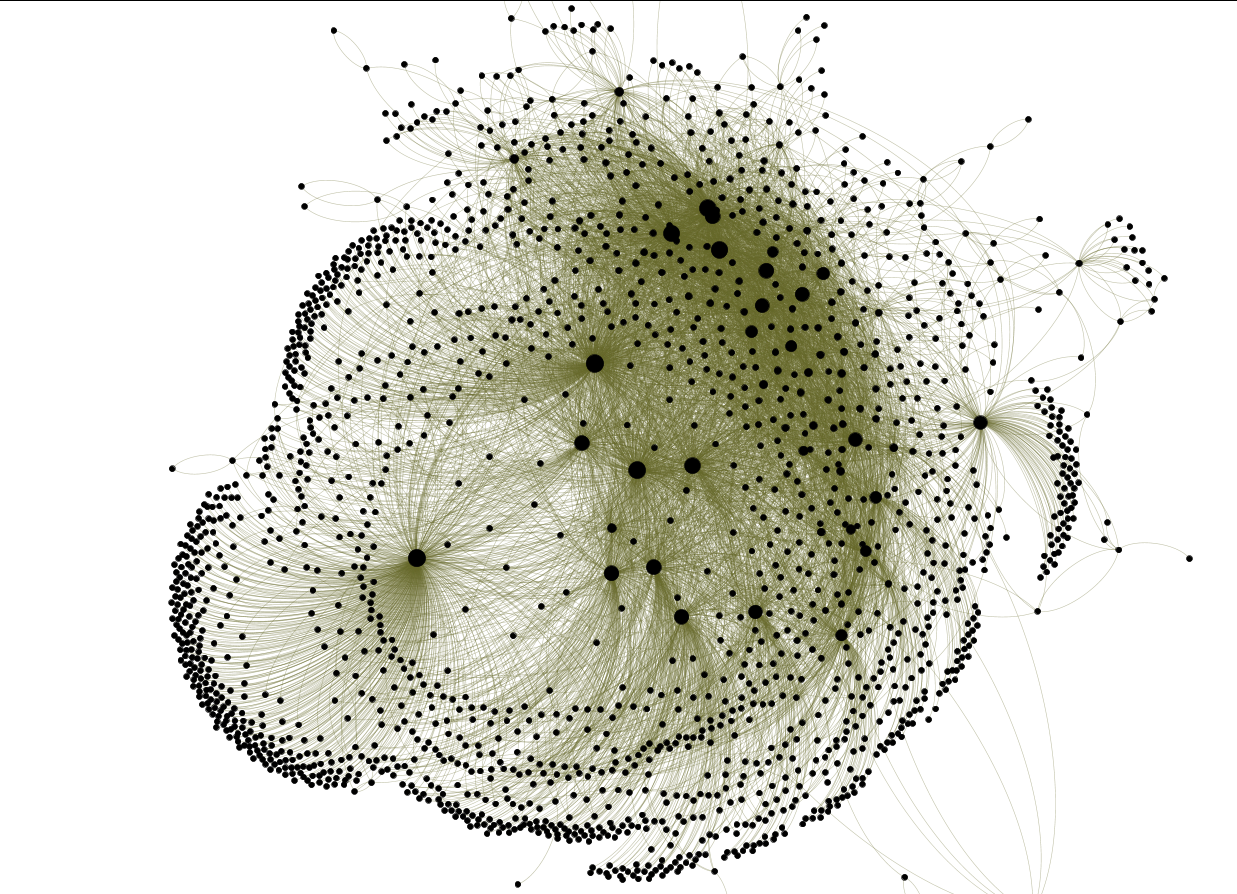
\includegraphics[width=12cm]{graphs/testnet_force.png}
	\vspace*{-0.4cm} 
	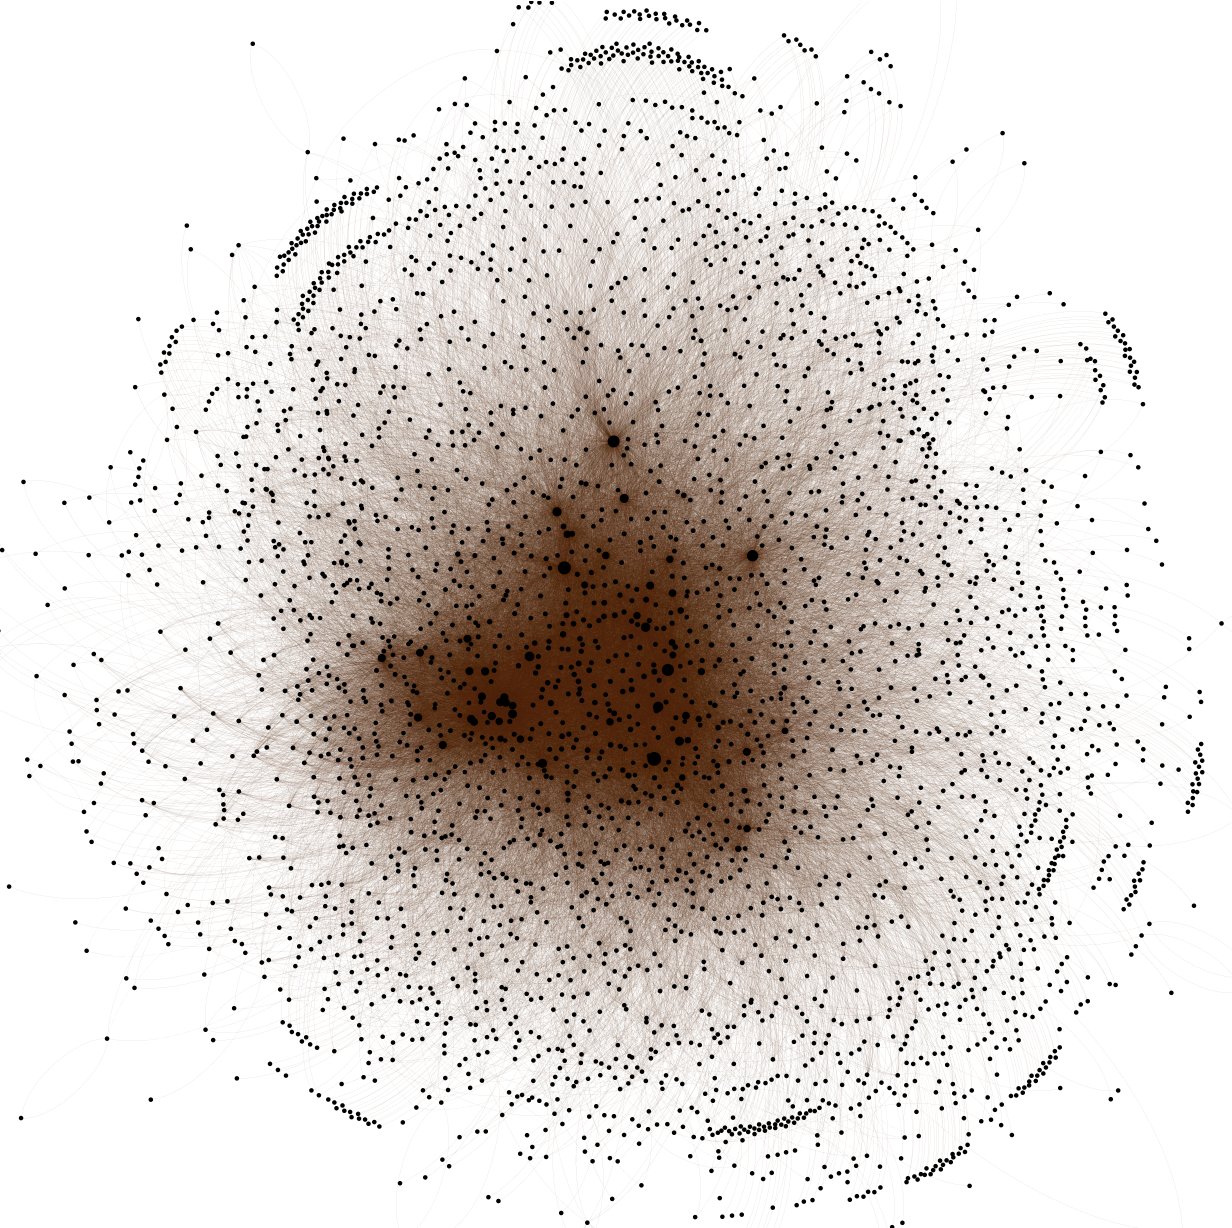
\includegraphics[width=13.6cm]{graphs/mainnet_force3.png}
	\caption{\textit{
			Shows testnet above and mainnet below as of 2019-02-25. Node size corresponds to degree, larger degrees to larger size. Positioning is a mix between Force Atlas and Fruchterman Raingold. Network data retrieved by running a c-lightning node and visualized with Gephi~\cite{repository:gephi}.}}
	\label{fig:topology}
	\hspace*{2mm} 	
\end{figure}
\newpage
\twocolumn

\section{Optimal fee price}

To determine the fee price, one could intuitively imagine that and increased fee price would yield higher fees but for less pairs as other paths may become shorter for pairs to route through. So the amount of shortest paths passing through a vertex must be calculated. In 1977 Freeman introduced a measurement named \textit{Betweenness Centrality}~\cite{freeman:betweenness:centrality} and defined it as

\[ g(v) = \sum_{s \neq v \neq d}\frac{\sigma_{sd}(v)}{\sigma_{sd}} \]

Where $\sigma_{sd}$ are all shortest paths from s to d and v is vertex. As the fee is determined on an edge basis the definition is altered to regard edges instead of vertices. 

It is possible to determine the optimal fee for an edge if some assumption, of the probability of all pairs transacting and the probability of the size of the transactions, are made. If a uniform probability over all pairs and that the shortest paths are used are assumed the optimal price for one payment size is given by

\[ x_{opt} \textrm{ is the optimal price } iff \]

\[ f: X \to \mathbb{Z} \textrm{ and } (\forall x \subseteq X)f(x_{opt}) \geqslant f(x) \textrm{ where }\]

\[ f(x) = x\sum_{s \neq e \neq d}\frac{\sigma_{sd}(e(x))}{\sigma_{sd}} \textrm{ and } \]

%\[ \sigma_{sd}(e(x)) =  \begin{cases}
%		n, & \text{if n shortest paths exists} \\
%          & \text{through $e$ with weight x.} \\
%		0, & \text{otherwise}
%	\end{cases} \]

\[ \sigma_{sd}(e(x)) =  \begin{cases}
 & \text{Is the sum of shortest } \\
 & \text{paths between $s$ and $d$} \\
& \text{through $e$ with weight x.} \\

\end{cases} \]


The $\sigma_{sd}$ represents the total amount of shortest paths between $s$ and $d$.
The function $f(x)$ behaves as seen in figure \ref{fig:fee_curve} for a fictitious generated graph. 

\begin{figure}[!htb]

	\centering
	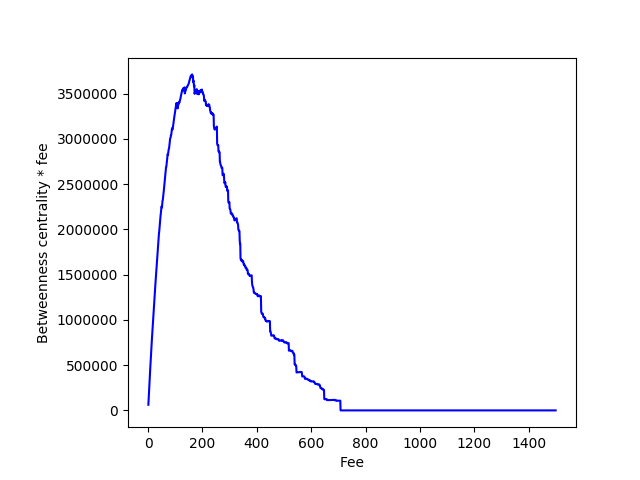
\includegraphics[width=8cm]{images/fee_curve.png}
	\caption{ Shows the betweenness centrality * fee / fee for an edge in a generated graph with 1000 vertices, 5000 edges, uniform weight distribution over 1-1500 and random attachment policy. It holds intuitively as for low fees, many shortest paths passes but procure small overall profits as the fee is small. The profits increases with the increase in fees until a point where the decrease in paths overtakes the increase in fees.
	}
	\label{fig:fee_curve}

\end{figure}

Freeman also defined a centrality measurement for whole graphs, it utilizes the betweenness centrality of every vertex and is thus brutal to calculate in practice for larger graphs. 

Efficient algorithms for edge betweenness centrality have been developed~\cite{brandes:betweenness:centrality:algorithm}. Although it is possible to run such an algorithm for each potential fee price to find the optima it would be very slow.
Instead the optimal fee price an for outgoing channel $e$, still holding the assumptions as before, may be calculated by following steps.

\begin{enumerate}
	\item Calculate the shortest path from all-to-all vertices without going through $e$ with either Floyd-Warshall~\cite{bakhtiar:floyd:warshall} or Johnson~\cite{johnson:shortest:path:sparse:network} obtaining table A.
	\item Calculate shortest path from the source of $e$, $V$-to-all explicitly going through $e$ with Dijkstra obtaining table D where $e$ weight set to 0.
	\item Retrieve the difference for all pairs between the all-to-all distance with the all-to-$V$-to-all distance, A[s][d] - (A[s][V] + D[d]). Throw away the negative values and produce a cumulative summation over the differences in a table H.
	\item Select $x_{opt}$ such that \[ \forall x (x H(x)) \leq x_{opt} H(x_{opt}) \]

\end{enumerate} 

Whenever Floyd-Warshall or Johnson should be used depends on the sparseness of G as Floyd-Warshall have a time complexity of

\[ O(V^3) \]

only dependent on vertices whereas Johnson

\[ O(V^2 log(V) + VE ) \]

depends on both edges and vertices. 

\subsection{Cost function}

As the previous solution naively assumes a fixed payment size, it's altered to encompass a payment size distribution.
The fee is proportional to the size of the payment, $F_B + F_P S$, thus the shortest path may be different for two different payment sizes. 
The problem is thus a combinatorial optimization problem,

\begin{equation*}
\hspace*{-0.5cm}	\max_{ x,y \in \mathbb{Z} } \sum_{\phi\in \rho} \rho(\phi) \sum_{a \neq b}
	\begin{cases}
	\Omega_{abe}(x, y, \phi) & \Omega_{abe}(x, y, \phi) < \sigma_{ab}(\phi)  \\
	0 & \Omega_{abe}(x, y, \phi) > \sigma_{ab}(\phi) \\
	\dfrac{\Omega_{abe}(x, y, \phi)}{\overline{\overline{\sigma_{ab}}} + 1} & \Omega_{abe}(x, y, \phi) = \sigma_{ab}(\phi)  \\
	\end{cases}
\end{equation*}

where $\Omega_{abe}(x, y, \phi)$, and $\sigma_{ab}(\phi)$ is given by

\begin{equation*}	
	\Omega_{abe}(x, y, \phi) = \Bigg( \sum_{c \in \sigma_{ae_s},\sigma_{e_db}} c_b + c_p\phi \Bigg) +
	x + y\phi 
\end{equation*}
\begin{equation*}
	\sigma_{ab}(\phi) = \Bigg( \sum_{c \in \sigma_{ab}} c_b + c_p\phi \Bigg)
\end{equation*}

where $\rho(\phi)$ is the fraction of payments size $\phi$. $e_s$, $e_d$ is edge source and destination nodes. $\sigma_{ab}$ is the edge set of the shortest path without going through $e$. $\overline{\overline{\sigma_{ab}}}$ is the number of paths equally short with the shortest path.

The function over $F_B$, $F_P$ in $f(x,y)$ follows the same pattern as over $F$ and is shown in Figure \ref{fig:cost:function:space}.

\begin{figure}[!htb]
	\vspace*{-0.0cm}
	\hspace*{0cm} 
	\centering
	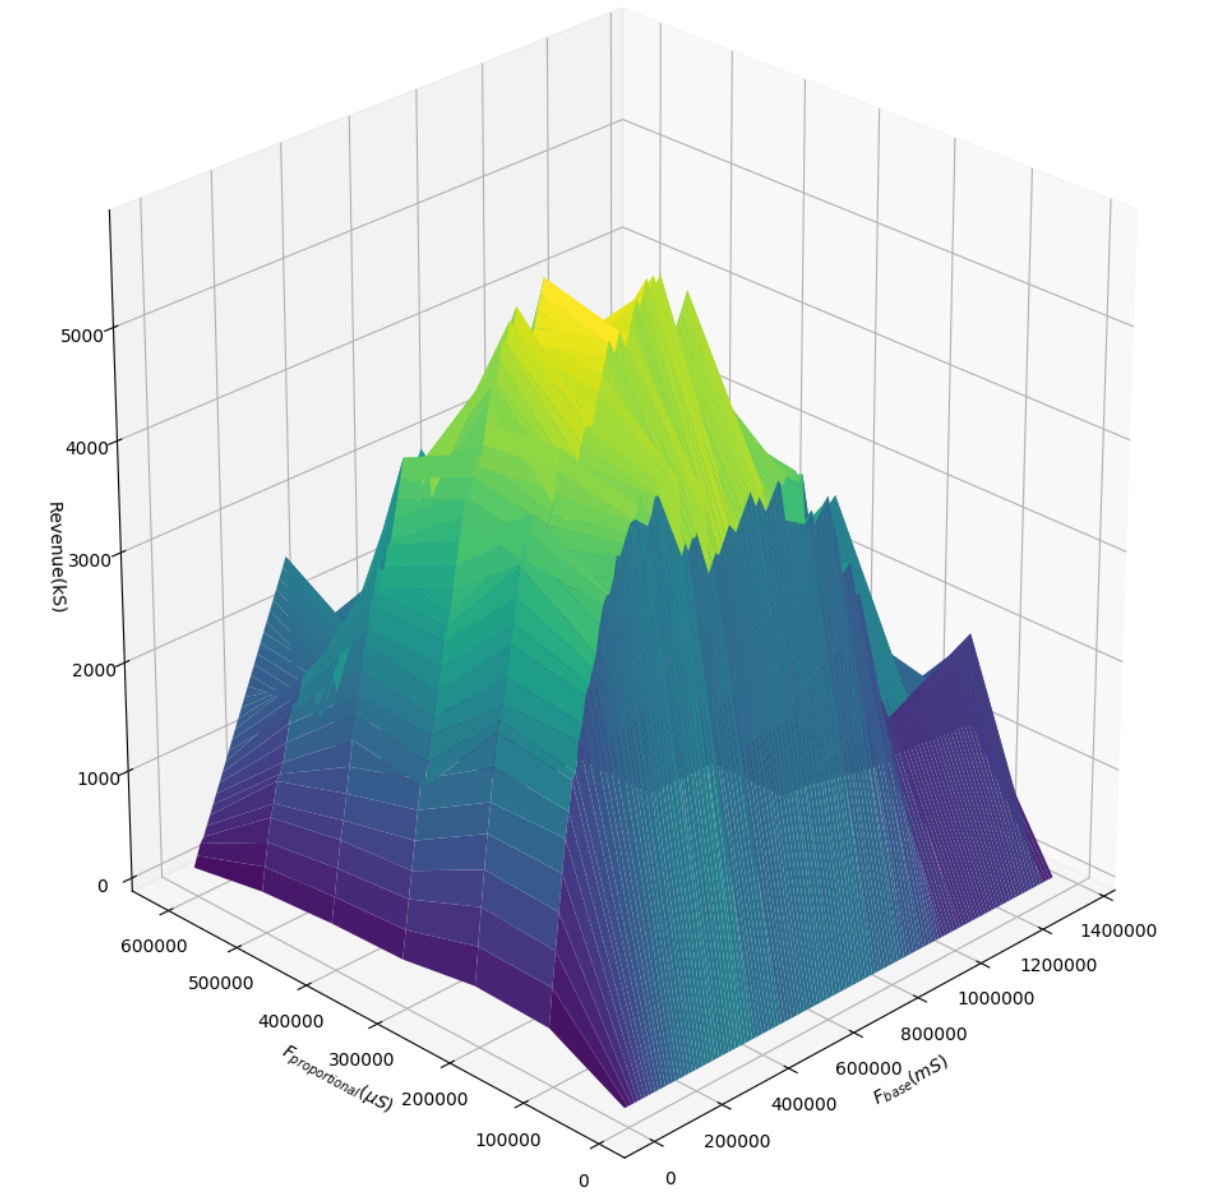
\includegraphics[width=9cm]{plots/price.png}
	\caption{Shows the relative revenue for a well connected edge over base and proportional fee when all other for a well connected edge in a generated graph. Assuming a uniform payment size distribution over 2,000 Satoshi - 2,000,000 Satoshi. }
	\label{fig:cost:function:space}
	\hspace*{2mm} 
\end{figure}

The combinatorial optimization problem may be solved similarly as before but with a modified Floyd-Warshall. Instead of the weights being integers, the weights are linear cost functions. For each new path the cumulative cost functions of edges in the paths are compared. If both $m$ and $k$ are greater than any previous found path it can be thrown away. If either $m$ or $k$ is greater their intersection can be stored as an index. If the intersections are stored in order only a logarithm of previously found paths need to be compared in the worst case. This finds all the shortest paths for each node pair over all transaction sizes. The paths may then be adjusted over intersection distance and payment size frequency, giving the optimal price.

This is however still a NP-hard problem and network growth will eventually make an exact solution infeasible. 

\subsection{Convert to probabilistic model}

It is cumbersome to calculate the optimal price for all edges; for simulation purposes it is completely infeasible. 

The price range given for an edge of well connected node used as a probabilistic model in quickly setting a good fee price. Given a simulation environment with defined strategies,  

\section{Topology and Preferential Attachment}

Setting fee price is only one aspect of a routing node, maybe more importantly is that of opening and closing channels.
As the protocol now stands\footnote{Is very plausible that that BIP66 may be activated allowing multi-sourced channels~\cite{bip:0118:sighash:noinput}} it only allows for single source funding of channels. There is a non negligible cost to opening channels and it would be very beneficial for a node if other nodes opened channels with it instead of the other way around. This is also a prerequisite to earn profit as otherwise the node may only earn back its own funding. 

Therefor the policies determining by which preferences each node takes into account to open channels is of interest. Further these policies also affects the topology of the network, the average shortest path and robustness in case of node failures.

\subsection{Traditional random models}

Random graphs have been studied extensively, specifically the Erdős–Rényi model~\cite{erdos:renyi:random:graphs}. An ER graph is created by denoting a graph $G_{n,N}$ with $n$ vertices and $N$ edges. The edges is then selected randomly from set of ${n \choose 2}$ possible edges. A common approach today is to write $G_{n,p}$ with $p$ being the probability of two vertices having an edge. It's difficult to justify LN behaving as an Erdős–Rényi graph as it allows for isolated points and there is no inherent age bias present. 

Callaway et al.~\cite{callaway:hopcraft:randomly:grown:graphs} added a phase transition to random graphs as to adjust for a supposed age bias. Consider $G_{n,\delta}$ where at first the graph is empty and for each time step a vertex v is added to the $G$ and an edge is selected over $G_v \choose 2$ with a probability $\delta$ until $G$ has $n$ vertices. $G_{n,\delta}$ would have on average $n\delta$ edges and since $n\delta < n$ it only produces sparse graphs. As before this may be difficult to apply to LN as a poorly connected graph would have high average paths and surely many payments would fail. It is however interesting to regard the \gls{degree distribution} compared to that of Erdős–Rényi as it's exponential given as

\begin{equation}
	p(k) = \dfrac{(2\delta)^k}{(1 + 2\delta)^{k+1}} 
	\label{eq:callaway}
\end{equation}
compared to Erdős–Rényi which is binomial

\begin{equation}
	p(k) = {n-1 \choose k} p^k(1-p)^{n-1-k} 
	\label{eq:erdos:renyi}
\end{equation}

as follows from definition as ${n-1 \choose k}$ are all possible combinations of k edges,  $p^k$ the probability of any combination taking place and $p^k(1-p)^{n-1-k}$ to exclude combinations of larger degree $k$.

Thus adding an age bias causes the characteristics of the \gls{degree distribution} to change as seen in Figure \ref{fig:callaway:erdos}.

\begin{figure}[!htb]
		\hspace*{-0.5cm} 
	\centering
	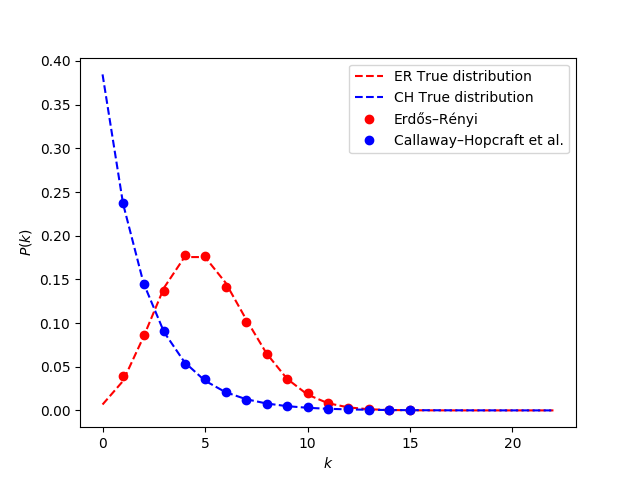
\includegraphics[width=9cm]{images/random_topology_degree_distribution.png}
	\caption{Shows the degree distribution for an Erdős–Rényi graph(\tikzcircle[red, fill=red]{2pt}) with n = 10,000, p = 0.0005 and its true distribution given by Equation \ref{eq:erdos:renyi}(\textcolor{red}{|}) compared to the degree distribution for a Callaway et al. graph(\tikzcircle[blue, fill=blue]{2pt})  with n = 10,000, $\delta$ = 0.8 and its true distribution given by equation\ref{eq:callaway}(\textcolor{blue}{|}).
	}
	\label{fig:callaway:erdos}
		\hspace*{2mm} 
\end{figure}

A more appropriate random model may be to consider $G_{n,m}$ where each time step $t$ a vertex is added to the graph and is connected with $m$ previous vertices and creates and edges when t < n. The probability of any previous vertex $i$ being selected is thus $p_i = \dfrac{m}{t_i}$. 
As a node may not be viewed as part of LN before edges are made, it's reasonable to assume a node creates edges as part of joining the network.

%[p(k) =  \begin{cases}
%& \prod_{i=1}^{k} 1 - \sum_{j=1}^{n-1} m \dfrac{1}{n^2},~\text{if}~m<k\\
%& 0,~~~~~~~~~~~~~~~~~~~~~~~~~\text{otherwise}

%\end{cases} \]

%\[ \prod_{i=1}^{k} 1 - \sum_{j=1}^{n-1} m \dfrac{1}{n^2} \sim 1 - m^k(\dfrac{1}{2})^k\]

\subsection{Scale free models}

In 1999 Barabási and Albert showed that many networks \gls{degree distribution} follows a power law and that the distribution was independent from scale, thus scale free~\cite{barabasi:albert:emergent:scaling}. Scale free networks follows a degree distribution of

\begin{equation}
	 p(k) \propto k^{-\gamma} 
	\label{eq:scale:free}
\end{equation}

and large network has been shown to follow this model. With notable networks of web hyperlinks having $\gamma_{www} = 2.1\pm 0.1$ and an actor collaboration graph having $\gamma_{actor} = 2.3\pm0.1$. Further suggestions have been made that network have an innate bias, as what has many links is well known and what is well known will receive many links - akin on the \textit{Pareto distribution}("80-20 rule") or the \textit{Matthew Effect}\footnote{As per KJB \texttt{Matthew 13:12 - For whosoever hath, to him shall be given, and he shall have more abundance: but whosoever hath not, from him shall be taken away even that he hath.}~\cite{king:james:bible}, after remark by Robert K. Merton~\cite{merton:matthew:effect}. }. 
A model was suggested to generate a scale free graph $G_{n, m}$ by starting with a graph with $m$ fully connected vertices, and for each time step adding a new vertex and creating $m$ edges with a bias towards vertices with high degree. The vertex may be said to have a preferred attachment and the probability of a vertex receiving an edge from the new vertex:

\[ \Pi(i) = \dfrac{k_i}{\sum_{j}^{}k_j} \]

Such a graph follows the scale free property with a $\gamma_{ba}$ = 2.9 and can be seen in Figure \ref{fig:scale_free}

\begin{figure}[!htb]
	\hspace*{-0.5cm} 
	\centering
	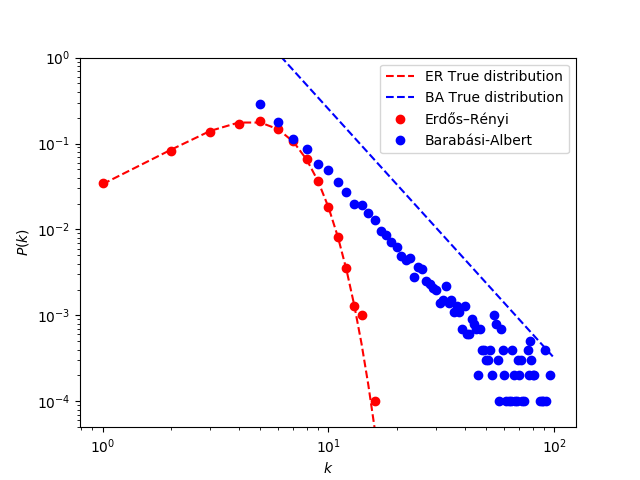
\includegraphics[width=9cm]{images/scale_free_degree_distribution.png}
	\caption{Shows the degree distribution for an Barabási–Albert graph(\tikzcircle[blue, fill=blue]{2pt}) with n = 10,000, m = 5 and the scale free\ref{eq:scale:free}(\textcolor{blue}{|}) with $\gamma$ = 2.9 compared Erdős–Rényi graph(\tikzcircle[red, fill=red]{2pt}) with n = 10,000, p = 0.0005 and its true distribution given by Equation \ref{eq:erdos:renyi}(\textcolor{red}{|}).
	}
	\label{fig:scale_free}
	\hspace*{2mm} 
\end{figure}

%modified barabasi

The actual degree distribution of the lightning network can be seen in Figure \ref{fig:real_network}.

\begin{figure}[!htb]
	\hspace*{-0.5cm} 
	\centering
	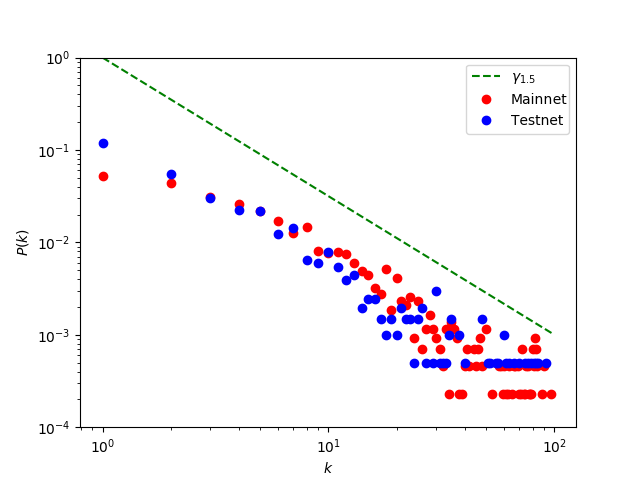
\includegraphics[width=9cm]{images/main-testnet_degree_distribution.png}
	\caption{Shows the degree distribution for both the Mainnet (\tikzcircle[red, fill=red]{2pt}) and Testnet (\tikzcircle[blue, fill=blue]{2pt})
		compared to the scale free function \ref{eq:scale:free}(\textcolor{black}{|}) with $\gamma$ = 1.5. The data is retrieved running a c-lightning node~\cite{repository:clightning} on 2019-03-21.
	}
	\label{fig:real_network}
	\hspace*{2mm}
\end{figure}
% Mainnet 4322 nodes and 21258 edges
% Testnet 2027 nodes, 8712 edges  

It should again be stated that the \gls{Lightning Network} is still in a very early state of it's development and most of the nodes and transactions over the network are made by enthusiasts trying it out. So the current state of the \gls{degree distribution} may indicate very little of future states. 

\subsection{Mediation-driven attachment}

Rather than explicitly attaching with a degree bias as with the Barabási-Albert model, Hassan et al.~\cite{hassan:islam:haque:mediation} have suggested a more subtle approach by attaching to a random neighbor of a randomly selected mediator node. Consider a node $i$ which degree $k_i$ and neighbors $1,2,...,k_i$ each having a degree of $k_1, k_2, ... k_{k_i}$ would thus have a probability $\Pi(i) \propto k_i$ and more explicitly,

\[ \Pi(i) = \dfrac{1}{N} \bigg\lbrack \dfrac{1}{k_1} + \dfrac{1}{k_2} + ... + \dfrac{1}{k_{k_1}} \bigg\rbrack = \dfrac{\sum_{j=1}^{k_i}\dfrac{1}{k_j}}{N} \]

They also show that it will lead to a scale free network, however the \gls{degree distribution} $\gamma$ is dependent on $m$ which differ from Barabási-Albert.

\subsection{Inverse Barabási-Albert}

%https://www.ncbi.nlm.nih.gov/pubmed/23005719

It may seem ridiculous that selecting nodes with low degree would be successful, however doing the opposite to the majority may be very promising. As these niche routes have considerably less competition, especially considering a node created at a large $t$ . If differentiation is a good strategy, this may capture it. The selection probability follows as, 

\[ \Pi(i) =  \dfrac{\dfrac{1}{k_i}}{\sum_{j}^{n} \dfrac{1}{k_j}} \]

where $\Pi(i)$ is the probability that node $i$ is selected with degree $k_i$

\subsection{Fitness models}

Node attachment may be influenced by fitness heuristics not intrinsic to the topology. E.g. Google overtook incumbent search engines having larger degree. The Bianconi-Barabasi model~\cite{bianconi:barabasi:fitness:network} was created to account for external heuristics.

\[ \Pi(i) = \dfrac{\eta_ik_i}{\sum_{j=1}^{n}\eta_jk_j}\ \]

By regarding the attachment probability growth over time,

\[ \dfrac{\partial k_i}{\partial t} = m \dfrac{\eta_ik_i}{\sum_{j=1}^{n}\eta_jk_j} \]

they are able to show that not all fitness distributions $\rho(\eta)$ results in a scale free network.

As there are many possible node heuristics beyond degree, e.g. capacity, availability and fee, these heuristics could be blend into the attachment models. 

Although Bianconi and Barabasi only studied fitness with the Barabási-Albert preferential attachment, it can however be added to the other models as well.

Time biased random model,
~
\[ \Pi(i) = \dfrac{\eta_i}{\sum_{j=1}^{n} \eta_j} \]

Inverse Barabasi-Albert model,

\[ \Pi(i) =  \dfrac{\eta_i\dfrac{1}{k_i}}{\sum_{j}^{n}\eta_j \dfrac{1}{k_j}} \]

Mediation driven attachment model,

\[ \Pi(i) = \dfrac{\eta_i\sum_{j=1}^{k_i}\dfrac{1}{k_j}}{N\sum_{j=1}^{n}\eta_j} \]

The $\eta_i$ can of course be a combination of heuristics $\eta_i = \phi_{i1} * \phi_{i2} * ... * \phi_{ik}$, scaled by constants in relation to each other and/or feature scaling normalized $\eta_i = c_1\rho(\phi_{i1}) * c_2\rho(\phi_{i2}) * ... * c_k\rho(\phi_{ik})$.

\subsection{Non degree fitness models}

All previous models have assumed that degree is relevant\footnote{Which is probable, it may though be useful to express it as any other heuristic.}. However it doesn't need to be expressed so explicitly, following from the Lognormal Fitness Attachment (LNFA)~\cite{bell:logonormal},

\[ \Pi(i) = \dfrac{\prod_{k=1}\phi_{ik}}{\sum_{j=1}^n\prod_{k=1} \phi_{jk}} = \dfrac{\eta_i}{\sum_{j=1}^{n} \eta_j} \]

which is evidently the same as the time biased random model. 

\subsection{Robustness}

Robustness is mainly regarded in terms of connectivity where reduction into sub components are measured when a percentage of either edges or nodes are removed. Usually the giant component, the largest component, as a percentage of the total network is indicative of partitions. As LN channels are virtual, edge connectivity doesn't make sense, which leaves node connectivity. Scale free networks are more robust than random networks\footnote{Note that time biased random networks is not considered here.} when nodes fail at random, but scale free networks are highly vulnerable if hubs are targeted~\cite{barabasi:robustness}. 

The current robustness of Mainnet is seen in Figure \ref{fig:accidental_failure} and \ref{fig:coordinated_attack} for accidental/random failures and targeted attacks respectively.

\vspace*{-0.45cm}
\begin{figure}[!htb]
	\hspace*{-1cm} 
	\centering
	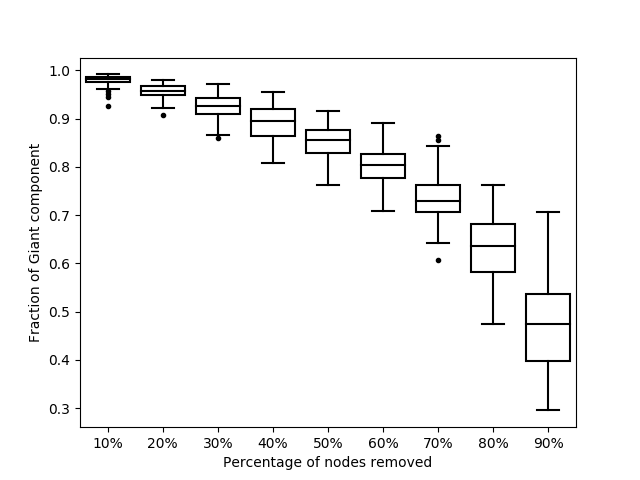
\includegraphics[width=9.5cm]{images/robustness_accidental.png}
	\caption{... . The data is retrieved running a c-lightning node~\cite{repository:clightning} on 2019-04-17.
	}
	\label{fig:accidental_failure}
	\hspace*{2mm} 
\end{figure}
\vspace*{-1.1cm}
\begin{figure}[!htb]
	\hspace*{-1cm} 
	\centering
	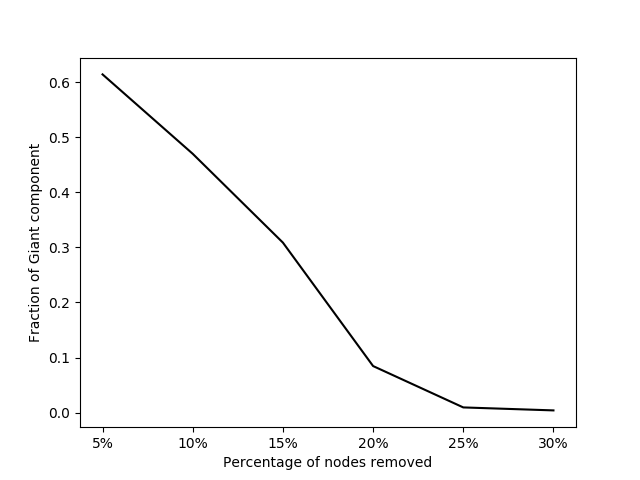
\includegraphics[width=9.5cm]{images/robustness_coordinated_mait.png}
	\caption{... . The data is retrieved running a c-lightning node~\cite{repository:clightning} on 2019-04-17.
	}
	\label{fig:coordinated_attack}
	\hspace*{2mm}
\end{figure}
\vspace*{-0.45cm}

\subsection{Average shortest path}

Each additional hop required in a payment path decreases the chance of having enough liquidity. It also increases failures in other dimensions, e.g. node compatibility and protocols levels below to fail. The average path growths at the same rate as the diameter, the longest shortest path between two nodes. For Erdős–Rényi the average path thus follows~\cite{watts:stragatz:small:networks},

\[ \ell \sim d \approx \dfrac{ln~N}{ln~pN} \]

For Barabási-Albert it is even shorter, with a double logarithmic correction it's considered 'ultrasmall'~\cite{cohen:havlin:ultrasmall},

\[ \ell \sim \dfrac{ln~N}{ln~ln~N} \]

The average path can be gathered empirically with Floyd-Warshall or Johnson,

\[ \ell = \dfrac{\sum_{i \neq j} \sigma_{ij}}{N(N-1)} \]

where $\sigma_{ij}$ is the length of the shortest path between $i$ and $j$.

\section{Re-balancing channels}

The ability to route payments is wholly dependent on having liquidity available. Constructing a route and pay to oneself is possible with the current protocol~[my impl ] which changes the balance of two edges for a fee. By doing a regular \textit{depth-first-search} cycles can be identified. For a route to be useful it must leave the two channels in a more balanced state than before. Here two simple heuristics are suggested. 

\subsection{Linear displacement}
\label{sec:linear:displacement}
If all increments towards the middle of the channel is considered equally valuable, then a the utility of a path is the combined liquidity towards balance per fee cost. Thus giving utility function,

\[ U(c) = \begin{cases} 
\dfrac{2|(B_{1S} - B_{1M})|}{f_c(|B_{1S} - B_{1M}|)}  & if~B_{1S} - B_{1M} < B_{2M} - B_{2S} \\ 
\\
\dfrac{2|(B_{2M} - B_{2S})|}{f_c(|B_{2M} - B_{2S}|)}  & otherwise
\end{cases} \]

where $B_{1S}$, $B_{2S}$ are the states of the out and in channels and $B_{1M}$, $B_{2M}$ their middles and $f$ is the total fee for cycle $c$. 

\[f_c(L) = \sum_{i=1}^{n} B_i + P_iL \]

with $B_i$ is the base fee, $P_i$ is the proportional fee for node $i$ in path $c$.

\subsection{Edge biased displacement}
\label{sec:edge:bias:displacement}

As a channel with most liquidity at one edge of the channel would only be able to route in one direction. Thus channels at one edge may be regarded with a bias in such that those channels would be preferred to re-balance. The bias can be stated explicitly to modify the linear displacement,

\[ U'(c) = U(c) \bigg(1,5 - \big(1 - \dfrac{B_{1S}}{2B_{1M}}\big) \bigg)^s \bigg(1,5 - \big(\dfrac{B_{2S}}{2B_{2M}}\big)\bigg)^s  \]

given a scalar $s$ by which the bias can by adjusted.

\subsection{Utility strategy scalar}

Each node can define how high the utility value must be to consider to re-balancing the channel by routing a payment to oneself.

\section{Funding and allocation strategies}

\section{Simulation}

The aforementioned strategies and a simulation environment were implemented in python 3.5 with extensive use of the networkx library.

The environment variables are tunable,  

and each players chosen strategies can be changed in a higher level configure file. Each strategy is discussed in detail in Appendix \ref{chapter:strategies} as well how a game may be created and simulated from altering the input file. Each set of strategies, under certain network dynamics may then be put into the same network to see which are stable and which are not. Similarly the emerging network is studied as successful strategies becomes more numerous at the hand of unsuccessful ones. 

% THE ADJUSTABLE SCALE FREE  http://www.uvm.edu/pdodds/files/papers/others/2002/holme2002a.pdf

% https://webusers.imj-prg.fr/~ricardo.perez-marco/publications/articles/antrouting3.pdf

% https://bitfury.com/content/downloads/whitepaper_flare_an_approach_to_routing_in_lightning_network_7_7_2016.pdf